\documentclass[11pt]{article}
\usepackage{paper_style}

\usepackage{lipsum}  %% Package to create dummy text (comment or erase before start)

%% ===============================================
%% Setting the line spacing (3 options: only pick one)
% \doublespacing
% \singlespacing
\onehalfspacing
%% ===============================================

\setlength{\droptitle}{-5em} %% Don't touch

% %%%%%%%%%%%%%%%%%%%%%%%%%%%%%%%%%%%%%%%%%%%%%%%%%%%%%%%%%%
% SET THE TITLE
% %%%%%%%%%%%%%%%%%%%%%%%%%%%%%%%%%%%%%%%%%%%%%%%%%%%%%%%%%%

% TITLE:
\title{This is the Title: I hope you like it
\thanks{Selected Paper prepared for presentation at the 201X Agricultural \& Applied Economics Association Annual Meeting}
}

% AUTHORS:
\author{First Author\\% Name author
    \href{mailto:firstauthor@ufl.edu}{\texttt{firstauthor@ufl.edu}} %% Email author 1
\and Second Author\\% Name author
    \href{mailto:secondauthor@ufl.edu}{\texttt{secondauthor@ufl.edu}} %% Email author 2
\and Third Author\\% Name author
    \href{mailto:thirdauthor@ufl.edu}{\texttt{thirdauthor@ufl.edu}}%% Email author 3
%\and Forth Author\\% Name author
%    \href{mailto:forthuthor@ufl.edu}{\texttt{forthuthor@ufl.edu}}%% Email author 4
    }

% DATE:
\date{\today}

% %%%%%%%%%%%%%%%%%%%%%%%%%%%%%%%%%%%%%%%%%%%%%%%%%%%%%%%%%%
% %%%%%%%%%%%%%%%%%%%%%%%%%%%%%%%%%%%%%%%%%%%%%%%%%%%%%%%%%%
\begin{document}
% %%%%%%%%%%%%%%%%%%%%%%%%%%%%%%%%%%%%%%%%%%%%%%%%%%%%%%%%%%
% %%%%%%%%%%%%%%%%%%%%%%%%%%%%%%%%%%%%%%%%%%%%%%%%%%%%%%%%%%
% ABSTRACT
% %%%%%%%%%%%%%%%%%%%%%%%%%%%%%%%%%%%%%%%%%%%%%%%%%%%%%%%%%%
% %%%%%%%%%%%%%%%%%%%%%%%%%%%%%%%%%%%%%%%%%%%%%%%%%%%%%%%%%%
{\setstretch{.8}
\maketitle
% %%%%%%%%%%%%%%%%%%
\begin{abstract}
% CONTENT OF ABS HERE--------------------------------------

\lipsum[1] %% Dummy text for abstract. Erase before use.

% END CONTENT ABS------------------------------------------
\noindent
\textit{\textbf{Keywords: }%
key1; key2; key3; key4.} \\ %% <-- Keywords HERE!
\noindent
\textit{\textbf{JEL Classification: }%
Q12; C22; D81.} %% <-- JEL code HERE!

\end{abstract}
}

% %%%%%%%%%%%%%%%%%%%%%%%%%%%%%%%%%%%%%%%%%%%%%%%%%%%%%%%%%%
% %%%%%%%%%%%%%%%%%%%%%%%%%%%%%%%%%%%%%%%%%%%%%%%%%%%%%%%%%%
% BODY OF THE DOCUMENT
% %%%%%%%%%%%%%%%%%%%%%%%%%%%%%%%%%%%%%%%%%%%%%%%%%%%%%%%%%%
% %%%%%%%%%%%%%%%%%%%%%%%%%%%%%%%%%%%%%%%%%%%%%%%%%%%%%%%%%%


% --------------------
\section{Introduction}
% --------------------

\lipsum[2-5] % Dummy text. Erase before write
\citet{Hardaker2004} % Example of citation. Erase before use


% --------------------
\section{Methodology}
% --------------------

\lipsum[7-9] % Dummy text. Erase before write
\citep{Chavas2015} % Example of citation. Erase before use


% --------------------
\section{Discussion and Conclusions}
% --------------------

\lipsum[14] % Dummy text. Erase before write


% %%%%%%%%%%%%%%%%%%%%%%%%%%%%%%%%%%%%%%%%%%%%%%%%%%%%%%%%%%
% %%%%%%%%%%%%%%%%%%%%%%%%%%%%%%%%%%%%%%%%%%%%%%%%%%%%%%%%%%
% REFERENCES SECTION
% %%%%%%%%%%%%%%%%%%%%%%%%%%%%%%%%%%%%%%%%%%%%%%%%%%%%%%%%%%
% %%%%%%%%%%%%%%%%%%%%%%%%%%%%%%%%%%%%%%%%%%%%%%%%%%%%%%%%%%
\medskip

\bibliography{references.bib}

\newpage

% %%%%%%%%%%%%%%%%%%%%%%%%%%%%%%%%%%%%%%%%%%%%%%%%%%%%%%%%%%
% %%%%%%%%%%%%%%%%%%%%%%%%%%%%%%%%%%%%%%%%%%%%%%%%%%%%%%%%%%
% TABLES
% %%%%%%%%%%%%%%%%%%%%%%%%%%%%%%%%%%%%%%%%%%%%%%%%%%%%%%%%%%
% %%%%%%%%%%%%%%%%%%%%%%%%%%%%%%%%%%%%%%%%%%%%%%%%%%%%%%%%%%

\begin{table}[H]
  \centering
  \caption{Example table of descriptive statistics of the main variables.}
  \label{tab:1}
  \scalebox{.8}{
    \begin{tabular}{rlrrrrrr}
    \hline
    \multicolumn{1}{c}{\textbf{Variables}} & \multicolumn{1}{c}{\textbf{Categories}} & \multicolumn{1}{c}{\textbf{Unit}} & \multicolumn{1}{c}{\textbf{Rep}} & \multicolumn{1}{c}{\textbf{Mean}} & \multicolumn{1}{c}{\textbf{St. Dev.}} & \multicolumn{1}{c}{\textbf{Min}} & \multicolumn{1}{c}{\textbf{Max}} \\ \hline \hline

    \multicolumn{1}{l}{Variable 1} & Category A & \multicolumn{1}{c}{\$} & \multicolumn{1}{c}{8} & 0     & 0     & 0     & 0 \\
          & Category B & \multicolumn{1}{c}{lb} & \multicolumn{1}{c}{8} & 22,411.20 & 6,325.90 & 13,819 & 31,201 \\
          & Category C & \multicolumn{1}{c}{\$} & \multicolumn{1}{c}{8} & 5,869.60 & 4,609.90 & -464.1 & 12,744.10 \\
    \multicolumn{1}{l}{Variable 2} & Category A & \multicolumn{1}{c}{\$} & \multicolumn{1}{c}{8} & 1,777.40 & 144.5 & 1,642.30 & 1,912.60 \\
          & Category B & \multicolumn{1}{c}{lb} & \multicolumn{1}{c}{8} & 21,444.80 & 5,146.90 & 15,096 & 28,032 \\
          & Category C & \multicolumn{1}{c}{\$} & \multicolumn{1}{c}{8} & 4,138.50 & 2,644.10 & 22.2  & 7,932.70 \\
    \multicolumn{1}{l}{Variable 3} & Category A & \multicolumn{1}{c}{\$} & \multicolumn{1}{c}{8} & 2,346.80 & 190.8 & 2,168.30 & 2,525.20 \\
          & Category B & \multicolumn{1}{c}{lb} & \multicolumn{1}{c}{8} & 18,343.30 & 2,460.70 & 15,269.00 & 21,524.10 \\
          & Category C & \multicolumn{1}{c}{\$} & \multicolumn{1}{c}{8} & 3,699.20 & 2,549.80 & 1,299.10 & 8,709.80 \\
    \multicolumn{1}{l}{Variable 4} & Category A & \multicolumn{1}{c}{\$} & \multicolumn{1}{c}{8} & 2,288.80 & 186.1 & 2,114.80 & 2,462.90 \\
          & Category B & \multicolumn{1}{c}{lb} & \multicolumn{1}{c}{8} & 23,450.40 & 4,172.50 & 20,045.00 & 32,363.00 \\
          & Category C & \multicolumn{1}{c}{\$} & \multicolumn{1}{c}{8} & 6,619.80 & 1,918.40 & 4,479.70 & 10,633.90 \\
\hline
          & CASE \#1 &       &       & 14    & 6.61  & 6.9   & 27.9 \\
          & CASE \#2 &       &       & 22.8  & 7.73  & 10.2  & 31.4 \\
    \hline
    \end{tabular}}
\end{table}%


% %%%%%%%%%%%%%%%%%%%%%%%%%%%%%%%%%%%%%%%%%%%%%%%%%%%%%%%%%%
% %%%%%%%%%%%%%%%%%%%%%%%%%%%%%%%%%%%%%%%%%%%%%%%%%%%%%%%%%%
% FIGURES
% %%%%%%%%%%%%%%%%%%%%%%%%%%%%%%%%%%%%%%%%%%%%%%%%%%%%%%%%%%
% %%%%%%%%%%%%%%%%%%%%%%%%%%%%%%%%%%%%%%%%%%%%%%%%%%%%%%%%%%

\begin{figure}[H]
    \centering
        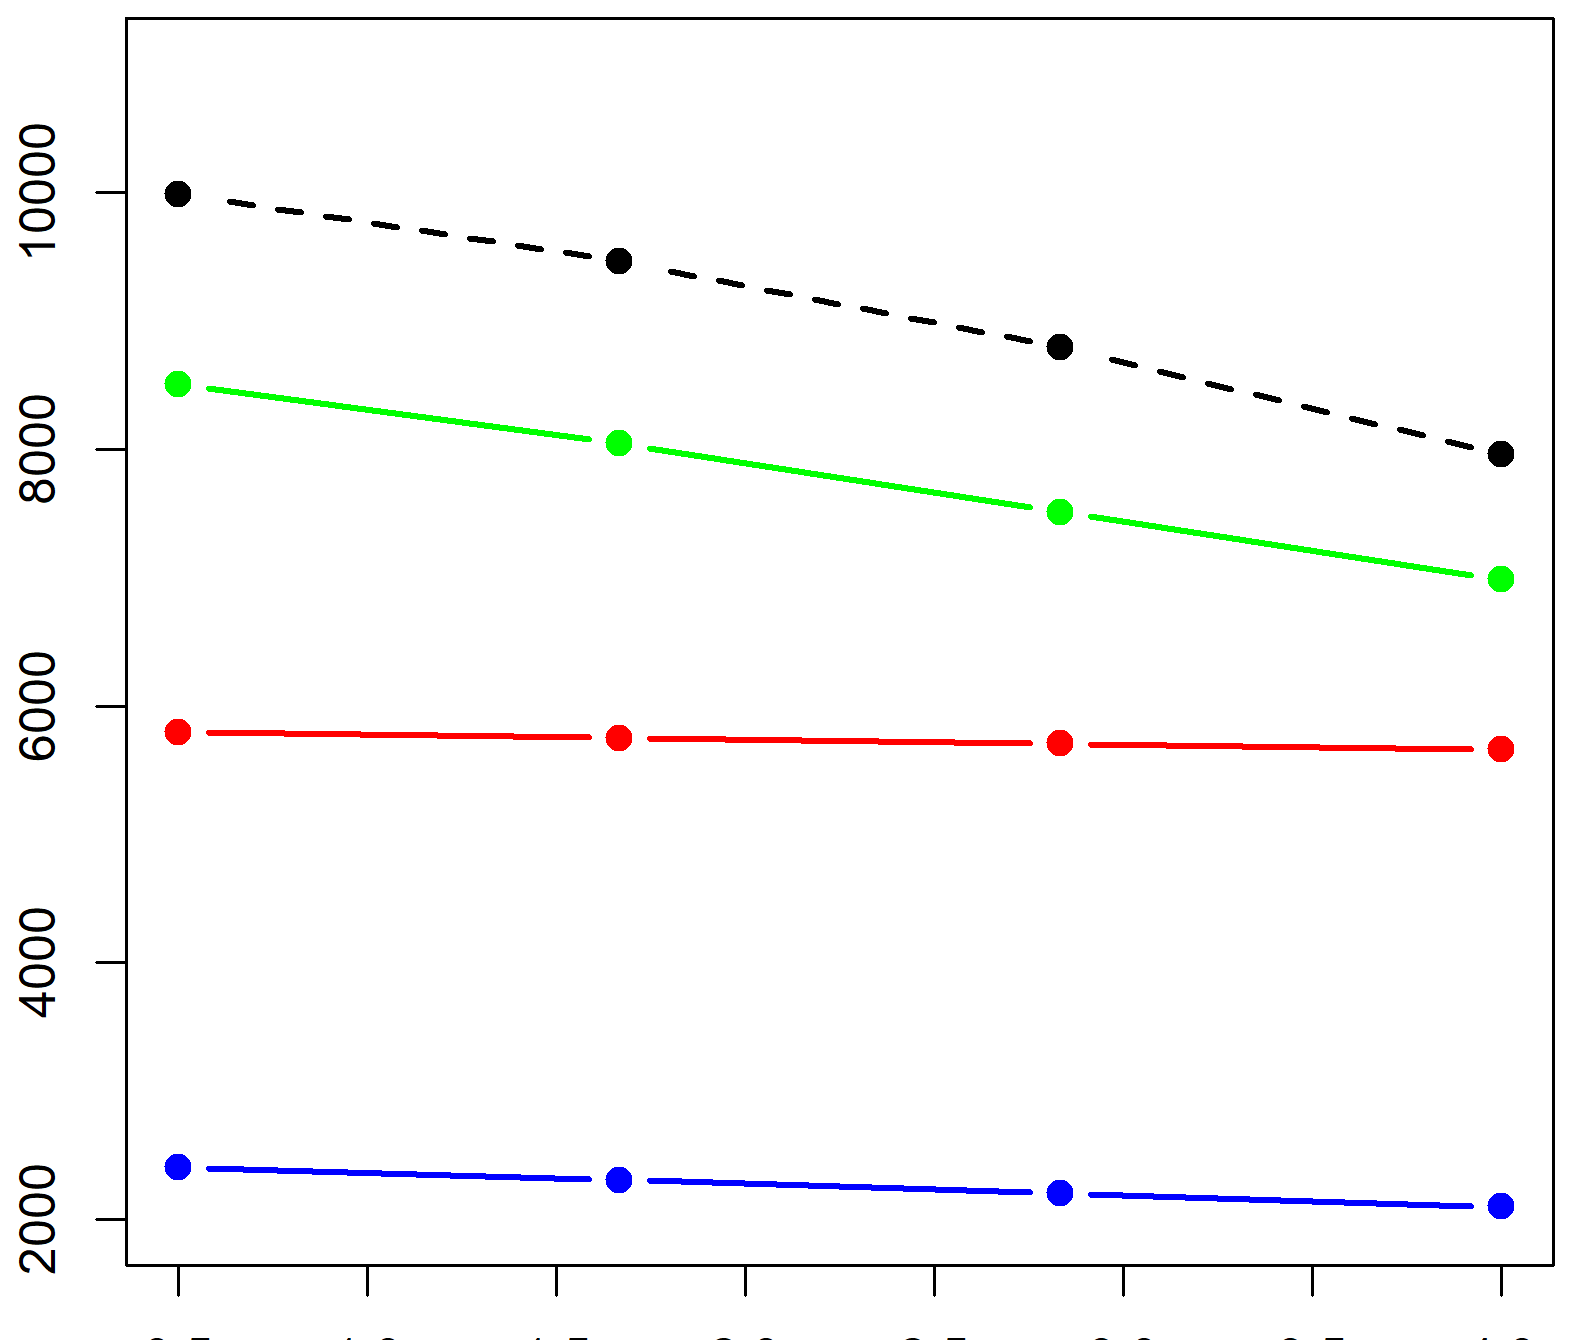
\includegraphics[scale=.6]{figures/example_figure.png}
    \caption{Example figure.}
    \label{fig:1}
\end{figure}

% ==========================
% ==========================
% ==========================


\end{document}
